%! Author = charon
%! Date = 2/8/24

\subsection{Übergabe von Daten als Parameter mithilfe von LD\_PRELOAD}\label{subsec: desocketing}
Wie bereits in Abschnitt~\ref{subsubsec:fuzzing-netzwerk-app} erläutert, ist das Fuzzen einer Netzwerkapplikation in dem bereits
implementierten Featureset von \gls{afl} nicht enthalten.
Hierzu kann eine Bibliothek selbst implementiert und als shared object kompiliert werden, sodass diese zum Start
der Applikation, mithilfe einer Umgebungsvariable namens \texttt{LD\_PRELOAD}, in die Applikation geladen wird.
Die Bibliothek beinhaltet eine eigene Implementierung der Syscalls \texttt{accept()}, \texttt{recv()}, \texttt{send()}
und \texttt{socket()}, welche die Funktionalität der bereits in libc-Bibliothek enthaltenen Funktionen überschreibt.
Um diese Funktionen effektiv für \gls{afl} nutzen zu können, müssen die genannten Syscalls so umgeschrieben werden, dass
Input, welcher über einen Netzwerksocket empfangen werden würde, stattdessen über die Eingabe von Dateien als Startparameter
übergeben wird.
Dieser Vorgang wird in der Fuzzing Community auch \textit{desocketing}~\cite{desocketing} genannt.
\gls{afl} besitzt bereits die Funktionalität ein shared object in Form einer \textit{.so} Datei in das zu untersuchende
Programm zu laden.
Unter \gls{afl} wird die Umgebungsvariable \texttt{AFL\_PRELOAD} genannt.\\
Bei diesem Binary werden jedoch keine Standard-Syscalls verwendet, sondern eine vom Hersteller implementierte Abstraktionsschicht,
welche die Funktionalität der Syscalls erweitert.
\begin{figure}[h]
    \frame{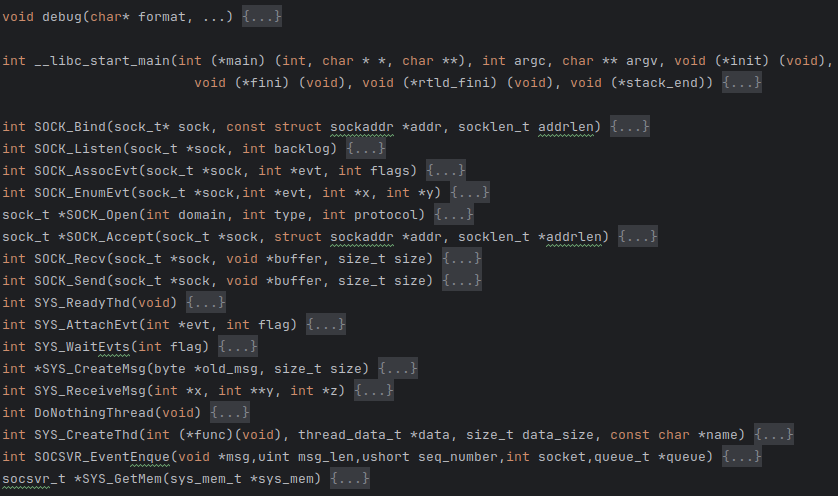
\includegraphics[width=\linewidth]{img/overwritten-funcs}}
    \caption{Zeigt die von Pahl überschriebenen Funktionen der preload Bibloiothek sockfuzz.so.
            Sie bestehen aus der vom Hersteller implementierten Abstraktionen der Standardfunktionen
            der libc Bibliothek.}\label{fig:overwritten-funcs}
\end{figure}\\
Das Ziel der Bibliothek ist es, das Überschreiben des \gls{tcp}-Sockets auf Port 7142, auf dem der gewünschte Netzwerkservice
läuft, sodass beim Fuzzen der Applikation keine Netzwerkanfragen lokal simuliert werden müssen.
Wichtig zu erwähnen ist hierbei, dass das direkte Senden von Daten an das Programm über das C \gls{cli} eine Performancesteigerung
um den Faktor der Größe 10 entspricht~\cite{afl-best-practice}.
Dies ist darauf zurückzuführen, dass weniger Overhead über den \gls{tcp}-Stack mitgegeben werden muss.
Ausschlaggebend bei dem Überschreiben der Abstraktionsschicht sind alle Funktionen, die nach einem Socket verlangen, sowie
die Funktion \texttt{\_\_libc\_start\_main()}.\\
Die Funktion \texttt{\_\_libc\_start\_main()}~\cite{libc-start-main} ist der Einstiegspunkt eines ausführbaren C-Programms und sorgt für das Initialisieren
der Laufzeitumgebung des Programms.
Ebenfalls ist die Funktion dafür verantwortlich die \texttt{main()} Funktion mit den zum Starten des Programms benötigten
Parametern (typischerweise \texttt{int argc} und \texttt{char *argv[]}) aufzurufen.\\
Der Einsprungspunkt muss überschrieben werden, damit die von \gls{afl} generierten Eingaben an das Programm als
Parameter zum Start des Programms übergeben werden können.
Dazu wird der \texttt{char *argv[]} Parameter der \texttt{main()} Funktion betrachtet.
Da der erste übergebene Parameter in C immer das Programm selbst ist, ist der zweite Parameter \texttt{argv[1]} der ausschlaggebende
Parameter.
Dieser über die Konsole übergebene Parameter wird bisher nicht von dem Programm verwendet und kann somit zur Übergabe der
Eingaben verwendet werden.
Als Nächstes wird die übergebene Datei an das Programm weitergegeben und gelangt weiter in den Calltree.
\gls{tcp}-Sockets unter auf \gls{unix} basierten Systemen arbeiten mit (Pseudo-)Dateien, welche einen Datenstrom repräsentieren.
Somit müssen alle Syscalls, welche auf den Socket 7142 verweisen, angepasst werden.
Sie sollen nicht mehr auf eine Datei, welche einen Socket repräsentiert, sondern auf die Datei, die von \gls{afl}
erzeugt wird, zugreifen.
Dafür soll die abstrahierte Version \texttt{SOCK\_Bind()} des \texttt{bind()} Syscalls überschrieben werden.
Er ist dafür verantwortlich, dass die Kommunikation über den richtigen Socket erfolgt.
